\chapter{SARANA PRASARANA KESEHATAN}
Pelayanan kesehatan kepada masyarakat harus didukung dengan sarana dan prasarana/ fasilitas yang memadai. Fasilitas pelayanan harus tersedia dan terdistribusi secara merata dalam jumlah dan jenis, serta berkualitas sesuai dengan kebutuhan masyarakat akan pelayanan kesehatan. 

\section{FASILITAS PELAYANAN KESEHATAN}
Undang-Undang Nomor 36 Tahun 2009 tentang Kesehatan menjelaskan bahwa fasilitas pelayanan kesehatan adalah suatu alat dan/atau tempat yang digunakan untuk menyelenggarakan upaya pelayanan kesehatan, baik promotif, preventif, kuratif, maupun rehabilitatif yang dilakukan oleh pemerintah, pemerintah daerah, dan/atau masyarakat. Penyelenggaraan Fasyankes diatur antara lain dalam Undang-undang Nomor 44 Tahun 2009 Tentang Rumah Sakit, Peraturan Menteri Kesehatan Republik Indonesia Nomor 75 Tahun 2014 Tentang Puskesmas serta Peraturan Menteri Kesehatan Republik Indonesia Nomor 56 Tahun 2014 Tentang Klasifikasi dan Perizinan Rumah Sakit.

\subsection{Rumah Sakit}
Rumah Sakit adalah institusi pelayanan kesehatan yang menyelenggarakan pelayanan kesehatan perorangan secara paripurna (promotif, preventif, kuratif dan rehabilitatif) yang menyediakan pelayanan rawat inap, rawat jalan dan gawat darurat\footnote{UU No 44 Tahun 2009, pasal 1 \& 4}. Rumah Sakit mempunyai fungsi :
\begin{enumerate}
  \item penyelenggaraan pelayanan pengobatan dan pemulihan kesehatan sesuai dengan standar pelayanan rumah sakit;
  \item penyelenggaraan pelayanan pengobatan dan pemulihan kesehatan sesuai dengan standar pelayanan rumah sakit;
  \item penyelenggaraan pendidikan dan pelatihan sumber daya manusia dalam rangka peningkatan kemampuan dalam pemberian pelayanan kesehatan; dan
  \item penyelenggaraan penelitian dan pengembangan serta penapisan teknologi bidang kesehatan dalam rangka peningkatan pelayanan kesehatan dengan memperhatikan etika ilmu pengetahuan bidang kesehatan;
\end{enumerate}

Jumlah Rumah Sakit di Kabupaten Belitung Timur pada tahun \tP adalah sebanyak 1 (Satu) unit Rumah Sakit Umum, yaitu RSUD Belitung Timur.

\subsection{Puskesmas}

Pusat Kesehatan Masyarakat (Puskesmas) adalah fasilitas pelayanan kesehatan yang menyelenggarakan upaya kesehatan masyarakat dan upaya kesehatan perseorangan tingkat pertama, dengan lebih mengutamakan upaya promotif dan preventif, untuk mencapai derajat kesehatan masyarakat yang setinggi-tingginya di wilayah kerjanya\footnote{Permenkes No 75 Tahun 2014, pasal 1}. Puskesmas sebagai salah satu jenis fasilitas pelayanan kesehatan tingkat pertama memiliki peranan penting dalam sistem kesehatan nasional, khususnya subsistem upaya kesehatan.

Jumlah Puskesmas menurut kecamatan di Kabupaten Belitung Timur tahun \tP adalah sebanyak 7 (enam) unit Puskesmas dengan rincian 4 (empat) unit Puskesmas Keperawatan yaitu Puskesmas Gantung, Puskesmas Simpang Pesak, Puskesmas Renggiang dan Puskesmas Kelapa Kampit, sedangkan 3 (dua) unit Puskesmas Non Keperawatan adalah Puskesmas Manggar, Puskesmas Mengkubang, dan Puskesmas Dendang.

\begin{figure}[H]
	\centering
	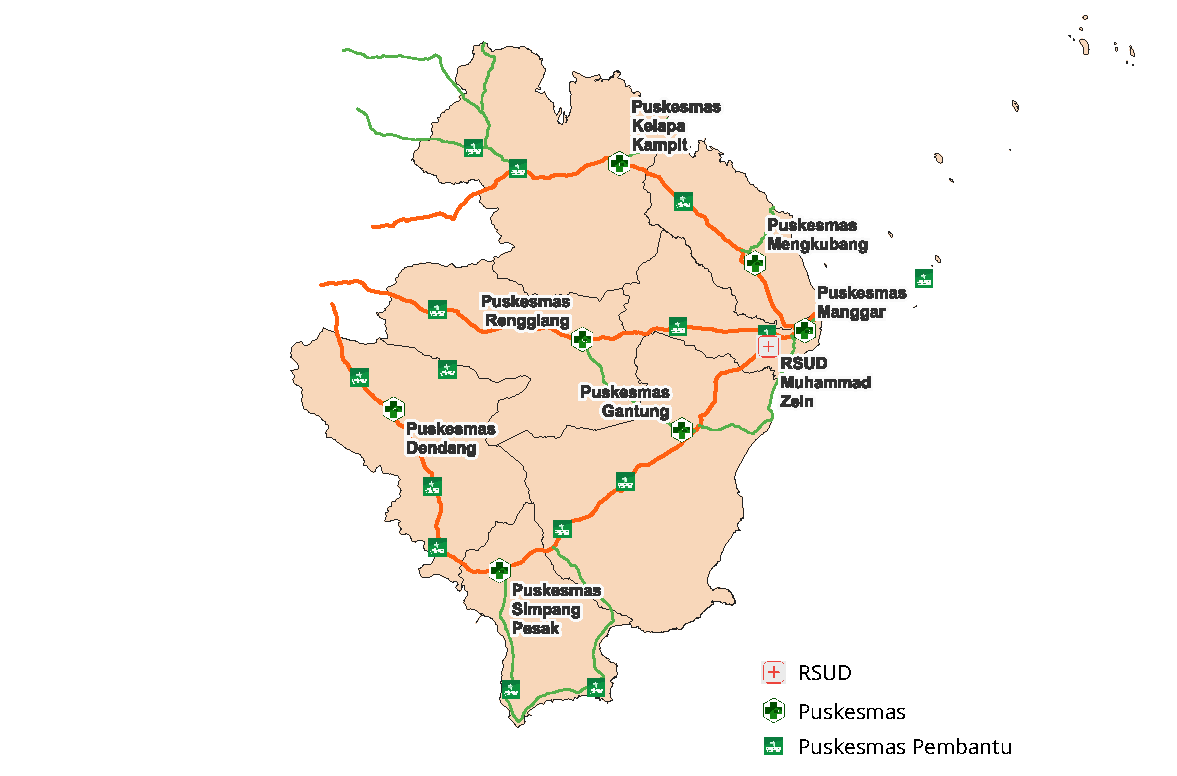
\includegraphics[width=0.85\textwidth]{bab_02/bab_02_01_petaFaskes}
	\caption{Lokasi Rumah Sakit, Puskesmas dan Puskesmas Pembantu di Kab. Belitung Timur}
	\label{fig:peta-puskesmas-rs}
\end{figure}

\subsection{Puskesmas Pembantu}

Puskesmas Pembantu merupakan jaringan pelayanan Puskesmas yang memberikan pelayanan kesehatan secara permanen di suatu lokasi dalam wilayah kerja Puskesmas\footnote{Permenkes No 75 Tahun 2014. pasal 40 ayat (2)}. Puskesmas  Pembantu merupakan bagian integral  Puskesmas, yang harus dibina secara berkala oleh Puskesmas.

Jumlah Puskesmas Pembantu di Kabupaten Belitung Timur pada tahun \tP adalah sebanyak 16 (Enam Belas) Pustu (\autoref{tab:Puskemas-dan-Pustu}).

\begin{table}[!ht]
\caption{Puskemas dan Jumlah Puskesmas Pembantu di Kab. Belitung Timur Tahun \tP}
\label{tab:Puskemas-dan-Pustu}
\centering{}%
\ra{1.3}

\begin{tabular}{lllr}
	\toprule
    No & Kecamatan & Puskesmas & Jumlah Puskesmas Pembantu\\
    \midrule
	1.                    & Manggar           & Manggar       & 3 \\
	\rowcolor{black!10}2. & Damar             & Mengkubang    & 1 \\
	3.                    & Gantung           & Gantung       & 3 \\
	\rowcolor{black!10}4. & Kelapa Kampit     & Kelapa Kampit & 2 \\
	5.                    & Simpang Renggiang & Renggiang     & 2 \\
	\rowcolor{black!10}6. & Simpang Pesak     & Simpang Pesak & 2 \\
	7.                    & Dendang           & Dendang       & 3 \\
    \midrule
    \multicolumn{2}{c}{Jumlah}                & 7             & 16\\
    \bottomrule
\end{tabular}
\end{table}

\section{AKSES DAN MUTU PELAYANAN KESEHATAN}
\subsection{Kunjungan Rawat Jalan dan Rawat Inap}
Kunjungan rawat jalan adalah kunjungan ke fasilitas pelayanan kesehatan tingkat pertama dan fasilitas pelayanan kesehatan rujukan tingkat lanjut milik pemerintah dan swasta untuk mendapatkan pelayanan kesehatan perseorangan yang meliputi observasi, diagnosa, pengobatan, rehabilitasi medik tanpa tinggal di ruang rawat inap untuk pertama kalinya dalam satu tahun tertentu. Kunjungan rawat jalan puskesmas termasuk kunjungan ke jaringan puskesmas, dalam gedung maupun luar gedung (puskesmas keliling, puskemas pembantu, bidan desa, pemeriksaan anak sekolah, dsb).
Kunjungan rawat inap adalah kunjungan ke fasilitas pelayanan kesehatan tingkat pertama dan fasilitas pelayanan kesehatan rujukan tingkat lanjut milik pemerintah dan swasta untuk mendapatkan pelayanan kesehatan perseorangan yang meliputi observasi, diagnosa, pengobatan, rehabilitasi medik, dan tinggal di ruang rawat inap untuk pertama kalinya dalam satu tahun tertentu.

Pada tahun \tP tercatat sebanyak 238.731 kunjungan di fasilitas layanan kesehatan di Kabupaten Belitung Timur. Sebanyak 157.915 kunjungan adalah ke fasilitas kesehatan milik pemerintah, sedangkan kunjungan ke fasilitas kesehatan milik swasta adalah sebanyak 80.816 kunjungan (\autoref{fig:Kunjungan-Faskes}).

Pada tahun \tP tercatat sebanyak 232.284 kali kunjungan rawat jalan dan 6.447 kunjungan rawat inap di fasilitas layanan kesehatan di Kabupaten Belitung Timur. Berdasarkan tingkat fasyankes, sebanyak 202.390 kunjungan adalah di Fasilitas Kesehatan Tingkat Pertama, sedangkan kunjungan di Fasilitas Kesehatan Tingkat Lanjutan adalah sebanyak 36.341 kunjungan (\autoref{fig:Kunjungan-Rawat}).

\begin{figure}[!htb]
    \centering{}
%    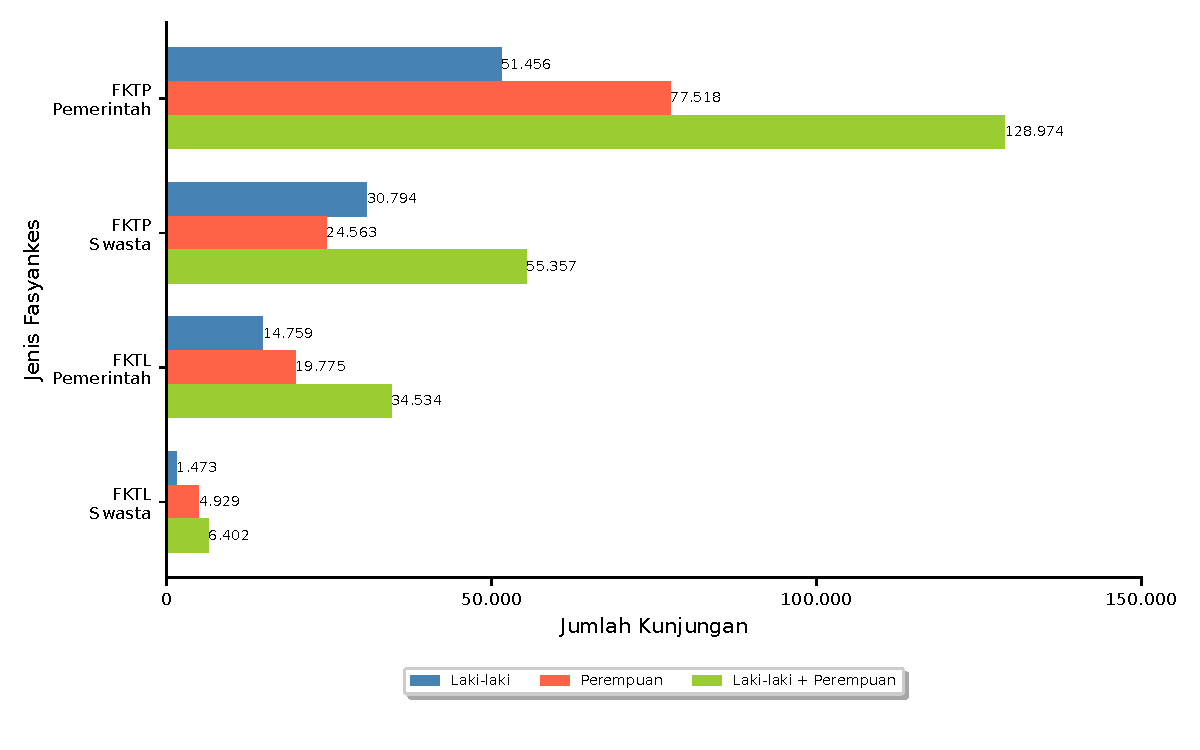
\includegraphics[width=0.9\textwidth]{bab_02/bab_02_1_kunjunganFaskes}
    \caption{Kunjungan Pasien Berdasarkan Jenis Faskes di Kab. Belitung Timur Tahun \tP}
    \label{fig:Kunjungan-Faskes}
\end{figure}

\begin{figure}[!htb]
    \centering{}
%    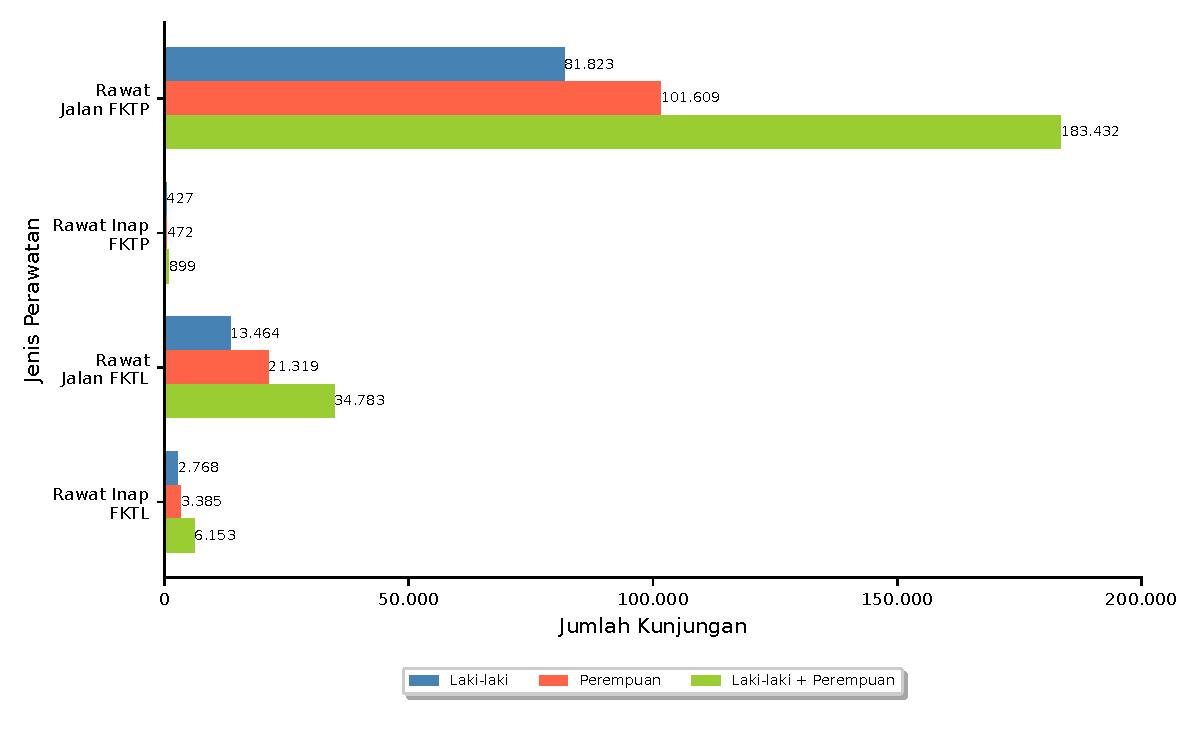
\includegraphics[width=0.9\textwidth]{bab_02/bab_02_2_rawat}
    \caption{Kunjungan Pasien Berdasarkan Jenis Perawatan di Kab. Belitung Timur Tahun \tP}
    \label{fig:Kunjungan-Rawat}
\end{figure}

\subsection{Kinerja Pelayanan Rumah Sakit}
Kinerja pelayanan rumah sakit dapat dinilai berdasarkan beberapa indikator, antara lain:
\begin{itemize}
 \item \emph{Gross Death Rate}(GDR), yaitu angka kematian umum untuk tiap-tiap 1.000 pasien keluar;
 \item \emph{Net Death Rate} (NDR), yaitu angka kematian ≥ 48 jam setelah dirawat untuk tiap-tiap 1.000 pasien keluar;
 \item \emph{Bed Occupancy Rate} (BOR), yaitu persentase pemakaian tempat tidur pada satu-satuan waktu tertentu;
 \item \emph{Bed Turn Over} (BTO), yaitu frekuensi pemakaian tempat tidur pada satu periode, berapa kali tempat tidur dipakai dalam satu satuan waktu;
 \item \emph{Turn Over Interval} (TOI), yaitu rata-rata hari tempat tidur tidak ditempati dari saat terisi ke saat terisi berikutnya; dan
 \item \emph{Average Length of Stay} (ALOS), yaitu rata-rata lama rawat (dalam satuan hari) seorang pasien.
\end{itemize}

Kinerja pelayanan rumah sakit di Kabupaten Belitung Timur pada tahun \tP dirangkum pada \autoref{tab:Kinerja-RS}.

\begin{table}[!ht]
\caption{Kinerja Pelayanan Rumah Sakit di Kab. Belitung Timur Tahun \tP}
\label{tab:Kinerja-RS}
\centering{}%
\ra{1.3}

\begin{tabular}{rlrr}
    \toprule
    No & Indikator                                          & Cakupan \tP       & Kondisi Ideal\\
    \midrule                                                
    1. & \emph{Gross Death Rate}                            & 66,27 per 1.000   & $\leq$ 45 per 1.000\\
    \rowcolor{black!10}2. & \emph{Net Death Rate}           & 30,80 per 1.000   & $\leq$ 25 per 1.000\\
    3. & \emph{Bed Occupancy Rate}                          & 47,02\%           & 60\% - 80\%\\
    \rowcolor{black!10}4. & \emph{Bed Turn Over}            & 46,18 kali        & 40 - 50 kali\\
    5. & \emph{Turn Over Interval}                          & 4,19 hari         & 1 - 3 hari\\
    \rowcolor{black!10}6. & \emph{Average Length of Stay}   & 3,76 hari         & 6 - 9 hari\\
    \bottomrule
\end{tabular}
\end{table}

\subsection{Ketersediaan Obat Esensial dan Vaksin IDL}
\subsubsection{Ketersediaan obat esensial}
Obat esensial adalah 40 item obat indikator yang merupakan obat pendukung Program Kesehatan Ibu dan Anak, Program Gizi, Program TB Paru, Program Malaria, serta obat pelayanan kesehatan dasar esensial dan terdapat di dalam Formularium Nasional.

Persentase Puskesmas dengan ketersediaan obat esensial adalah persentase Puskesmas yang memiliki ketersediaan minimal 80\% dari 40 item obat indikator pada saat dilakukan pemantauan terhadap
seluruh puskesmas yang melaporkan data. Laporan yang disampaikan yaitu laporan pada bulan November atau laporan bulan terakhir pada tahun pelaporan.

Pada tahun \tP terdapat 100\% Puskesmas yang memenuhi ketersediaan obat esensial di Kabupaten Belitung Timur.

\subsubsection{Ketersediaan vaksin IDL}
Vaksin Imunisasi Dasar Lengkap (IDL) terdiri dari Vaksin Hepatitis B, Vaksin BCG, Vaksin DPT-HB-HIB, Vaksin Polio dan Vaksin Campak/Campak Rubella.

Ketersediaan vaksin IDL adalah persentase Puskesmas yang memiliki vaksin IDL pada saat dilakukan pemantauan terhadap seluruh puskesmas yang melaporkan data. Laporan yang dimasukkan yaitu laporan pada bulan November atau laporan bulan terakhir pada tahun pelaporan.

Pada tahun \tP terdapat 100\% Puskesmas yang memenuhi ketersediaan vaksin IDL di Kabupaten Belitung Timur.


\section[UKBM]{UPAYA KESEHATAN BERSUMBERDAYA MASYARAKAT (UKBM)}% for title and page
\sectionmark{UKBM} %for header
\subsection{Posyandu}
Posyandu adalah salah satu bentuk Upaya Kesehatan Bersumberdaya Masyarakat (UKBM) yang dikelola dan diselenggarakan dari, oleh, untuk, dan bersama masyarakat guna memberdayakan masyarakat dan memberikan kemudahan kepada masyarakat dalam memperoleh pelayanan kesehatan dasar untuk mempercepat penurunan angka kematian ibu, bayi, dan balita. Posyandu melayani kegiatan berupa penimbangan bayi dan balita, pemberian imunisasi, konsultasi kesehatan dan Pemberian Makanan Tambahan (PMT).

Posyandu aktif mengalami perubahan definisi operasional pada tahun \tP , yaitu menjadi posyandu aktif adalah jumlah posyandu purnama dan mandiri. Jumlah Posyandu di Kabupaten Belitung Timur tahun \tP adalah sebanyak 133 posyandu aktif dari total 134 unit posyandu (\autoref{fig:Posyandu-Aktif}).

\begin{figure}[H]
	\centering{}
%	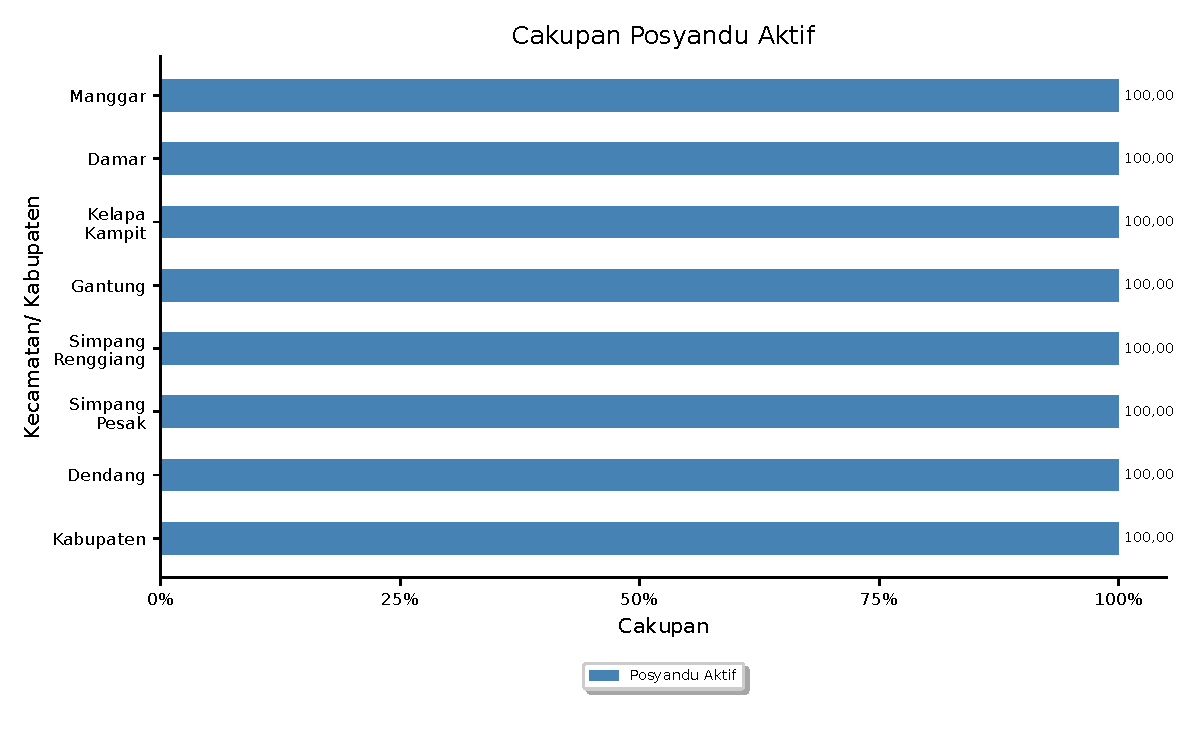
\includegraphics[width=0.9\textwidth]{bab_02/bab_02_3_posyandu}
	\caption{Persentase Posyandu Aktif di Kab. Belitung Timur Tahun \tP}
	\label{fig:Posyandu-Aktif}
\end{figure}

\subsection{Posbindu PTM}
Posbindu PTM adalah suatu upaya kesehatan berbasis bersumberdaya masyarakat (UKBM) dalam pencegahan dan pengendalian Penyakit Tidak Menular (PTM) melalui kegiatan skrining kesehatan/ deteksi dini faktor risiko PTM, intervensi/ modifikasi faktor risiko PTM serta monitoring dan tindak lanjut faktor risiko PTM bersumber daya masyarakat secara rutin dan berkesinambungan.

Jumlah Posbindu PTM di Kabupaten Belitung Timur tahun \tP adalah sebanyak 62 Posbindu PTM. %(\autoref{tab:Posyandu-Posbindu-di-Kab}).
